 \documentclass{article}
    \usepackage{amsmath}
    \usepackage[utf8]{inputenc}
    \usepackage[english]{babel}
    \usepackage{color}
    \usepackage{graphicx}
    \usepackage{enumitem}
    \usepackage{incgraph}
    \hyphenpenalty=10000
    \exhyphenpenalty=10000
    % \usepackage[T1]{fontenc}
    % \usepackage{geometry}
    \usepackage[top = 2cm, bottom = 2cm]{geometry}
    
    \usepackage[familydefault,light]{Chivo} 
    \usepackage[T1]{fontenc}
    
    \setlength{\parindent}{4em}
    \setlength{\parskip}{2em}
\renewcommand{\baselinestretch}{1.5}
    \usepackage{graphicx}
    
    \usepackage{listings}
    \usepackage{color}
    
    \definecolor{dkgreen}{rgb}{0,0.6,0}
    \definecolor{gray}{rgb}{0.5,0.5,0.5}
    \definecolor{mauve}{rgb}{0.58,0,0.82}
    
    \lstset{frame=tb,
      language=ocaml,
      aboveskip=3mm,
      belowskip=3mm,
      showstringspaces=false,
      columns=flexible,
      basicstyle={\small\ttfamily},
      numbers=none,
      numberstyle=\tiny\color{gray},
      keywordstyle=\color{blue},
      commentstyle=\color{dkgreen},
      stringstyle=\color{mauve},
      breaklines=true,
      breakatwhitespace=true,
      tabsize=3
    }
    
    \title{COL 783 \\ Assignment 4}
    \author{Rajbir Malik \\ 2017CS10416}
    
    \begin{document}
    
    \maketitle

%  Starting page
% -------------------------------------------------------
% -------------------------------------------------------
    \begin{center}
    \Large{\underline{\textbf{Robust Form Processing}}}
    \end{center}
    \subsection*{Overview}
    The assignment required us to process some forms in different natural settings, and trying to extract meaningful information from the forms.\\
    Being much open ended, we had the opportunity to try various procedures to get the task done. I was, after many attempts, able to come up with a "mostly" automated process to get the required information.\\ I have presented this approach and explained the procedure in the upcoming report. I've also discussed another approach that was reasonable to some scale, but couldn't be scaled, by me, to the desired level.
% -------------------------------------------------------
% -------------------------------------------------------
% Topic I
    \pagebreak
    \subsection*{Image Alignment}
% -------------------------------------------------------
    I worked upon the\e lines of a standard form scanner, to get all the input images aligned correctly.\\
    Having created a template-default form, I used it as reference to get the ideal warp-perspective for the input image, with the help of descriptor-matching.\\
    The exact pseudo-code for the same has been described below...\\
    \begin{lstlisting}
def image_alignment(_input_image, _template):
    - Create ORB Descriptor
    - Get Key-Points and Descriptors
    - Match the features
    - Filter the matches, to get the ideal ones for mapping
    - Using keypoints, discover ideal homography
    - Use the homography, and warp the input image
    - Return the warped image
    \end{lstlisting}
\textbf{Results}\\
    The results for alignment procedure were quite-impressive, achieveing as good as 99\% accuracy for \texttt{printouts} and \texttt{scanned} and reasonable results for \texttt{boooklets}. Perhaps, if I could find ideal templates for booklets as well (which I couldn't), then there too a decent result may have been procured.\\
    Further, I present the results of alignment on all the categories (2 of each kind).\\
\textbf{Another Approach}\\
    I also tried with a much simpler approach earlier, which involved finding the lines using \texttt{Canny-Edge Detector} and then using \texttt{Hough-Transform} to get the angle at which maximum no. of lines appeared.\\ This approached, though naive seemed to work sensibly for \texttt{scanned}-images, but failed badly for both \texttt{printouts} and \texttt{boooklets}. So, I was compelled to drop the idea.
\pagebreak
% -------------------------------------------------------

    \begin{figure}[!htb]
    %
    \minipage{\textwidth}
    \begin{center}
      \includegraphics[scale=.55]{4/lib/_data5/}
      \caption{Face}
    \end{center}
    \endminipage \hfill
    \end{figure}
% -------------------------------------------------------    
    \\[5pt]\textbf{Another example}\\
    Here, I've smoothened the merge even further, by using different splines, each increasingly smoother.\\
    This lead to increasing compatibility (or acceptability) of merge.\\[3pt]
% -------------------------------------------------------
    \begin{figure}[!htb]
    %
    \minipage{0.45\textwidth}
    \begin{center}
      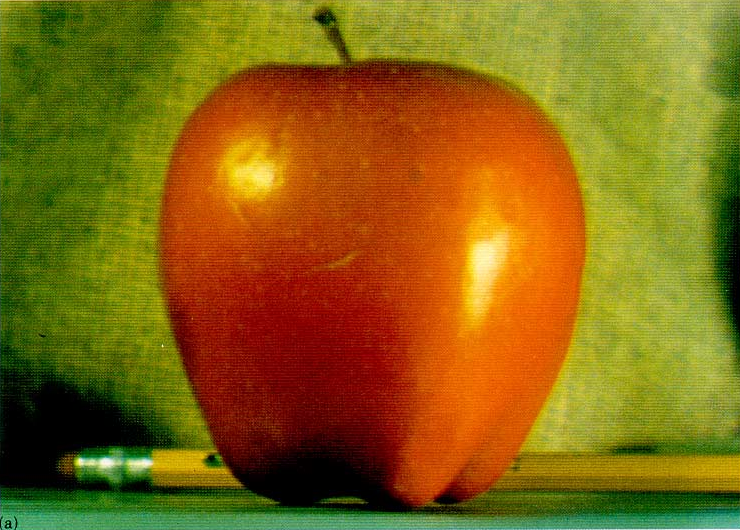
\includegraphics[scale=.35]{./blending/ao/apple.png}
      \caption{Apple}
    \end{center}
    \endminipage \hfill
    %
    \minipage{0.45\textwidth}
    \begin{center}
      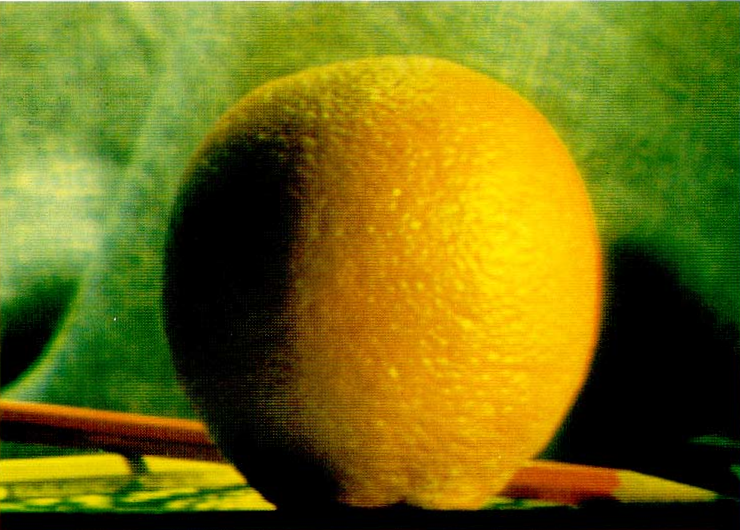
\includegraphics[scale=.35]{./blending/ao/orange.png}
      \caption{Orange}
     \end{center}
    \endminipage \hfill
    %
    \end{figure}

% -------------------------------------------------------
    \pagebreak
% -------------------------------------------------------
    \begin{figure}[!htb]
    \minipage{0.5\textwidth}
      \fbox{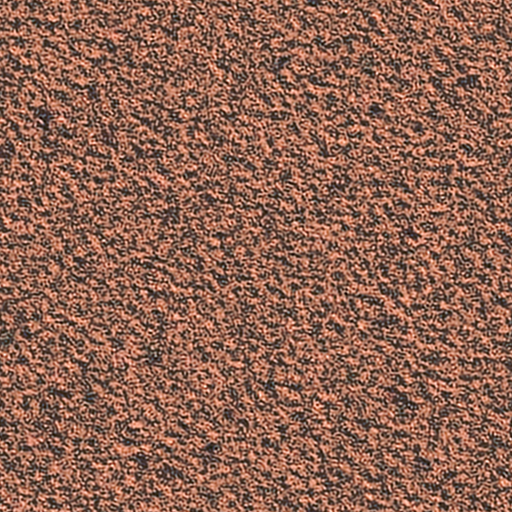
\includegraphics[scale=.25]{./blending/ao/1.png}}
      \caption{Merger}
    \endminipage \hfill
    %
    \minipage{0.5\textwidth}
      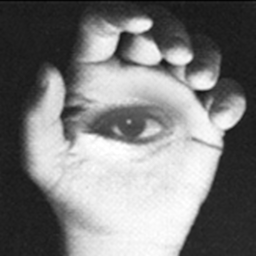
\includegraphics[scale=.3]{./blending/ao/final_1.png}
      \caption{Merge}
    \endminipage \hfill
    %
    \end{figure}

% -------------------------------------------------------
    
    \begin{figure}[!htb]
    \minipage{0.5\textwidth}
      \fbox{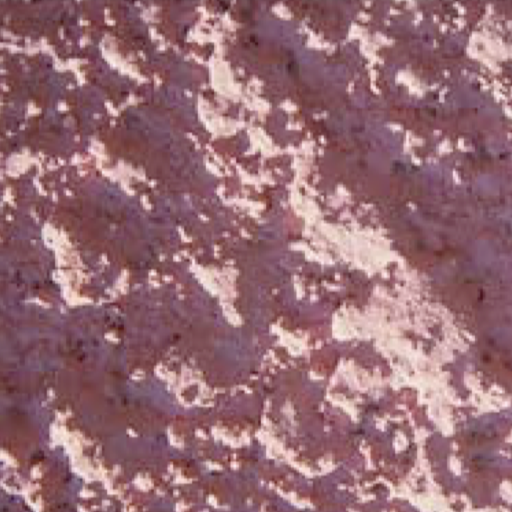
\includegraphics[scale=.25]{./blending/ao/2.png}}
      \caption{Merger}
    \endminipage \hfill
    %
    \minipage{0.5\textwidth}
      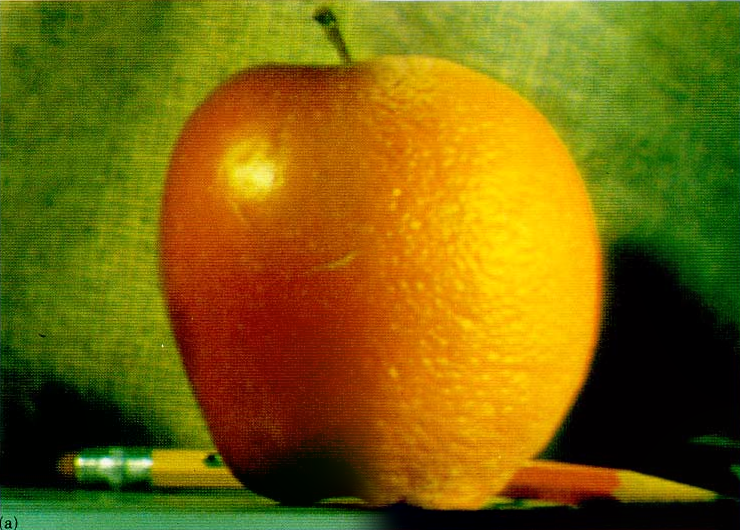
\includegraphics[scale=.3]{./blending/ao/final_2.png}
      \caption{Merge}
    \endminipage \hfill
    %
    \end{figure}

% -------------------------------------------------------
    \begin{figure}[!htb]
    \minipage{0.5\textwidth}
      \fbox{
\includegraphics[scale=.25]{./blending/ao/3.png}}
      \caption{Merger}
    \endminipage \hfill
    %
    \minipage{0.5\textwidth}
      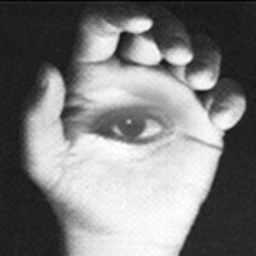
\includegraphics[scale=.3]{./blending/ao/final_3.png}
      \caption{Merge}
    \endminipage \hfill
    %
    \end{figure}
    
% ------------------------------------------------------- 
    \pagebreak
    \textbf{Another example}
    
    \begin{figure}[!htb]
    \minipage{0.5\textwidth}
      \fbox{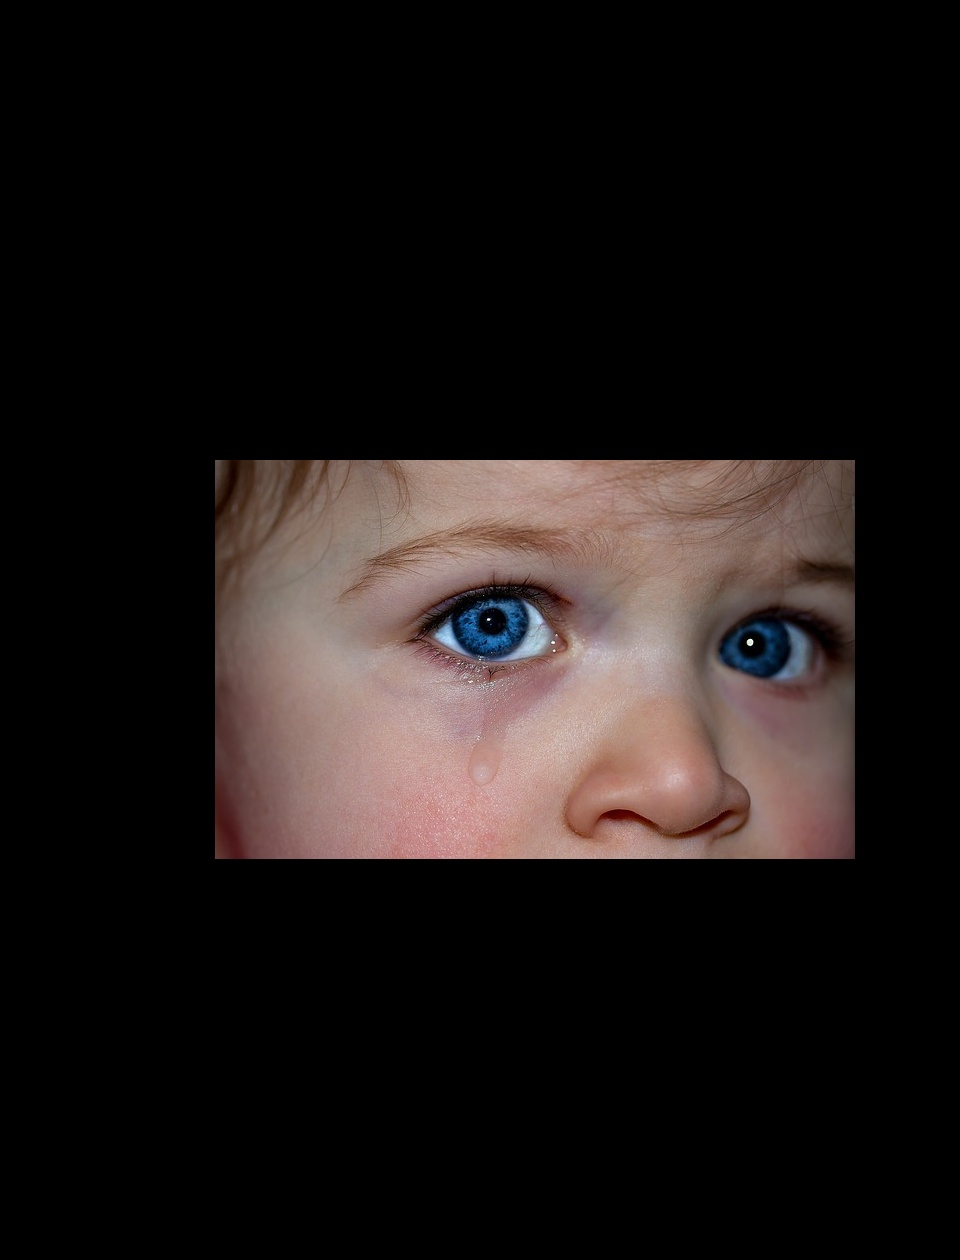
\includegraphics[scale=.20]{3/.report/blending/et/eye.png}}
      \caption{Merger}
    \endminipage \hfill
    %
    \minipage{0.5\textwidth}
      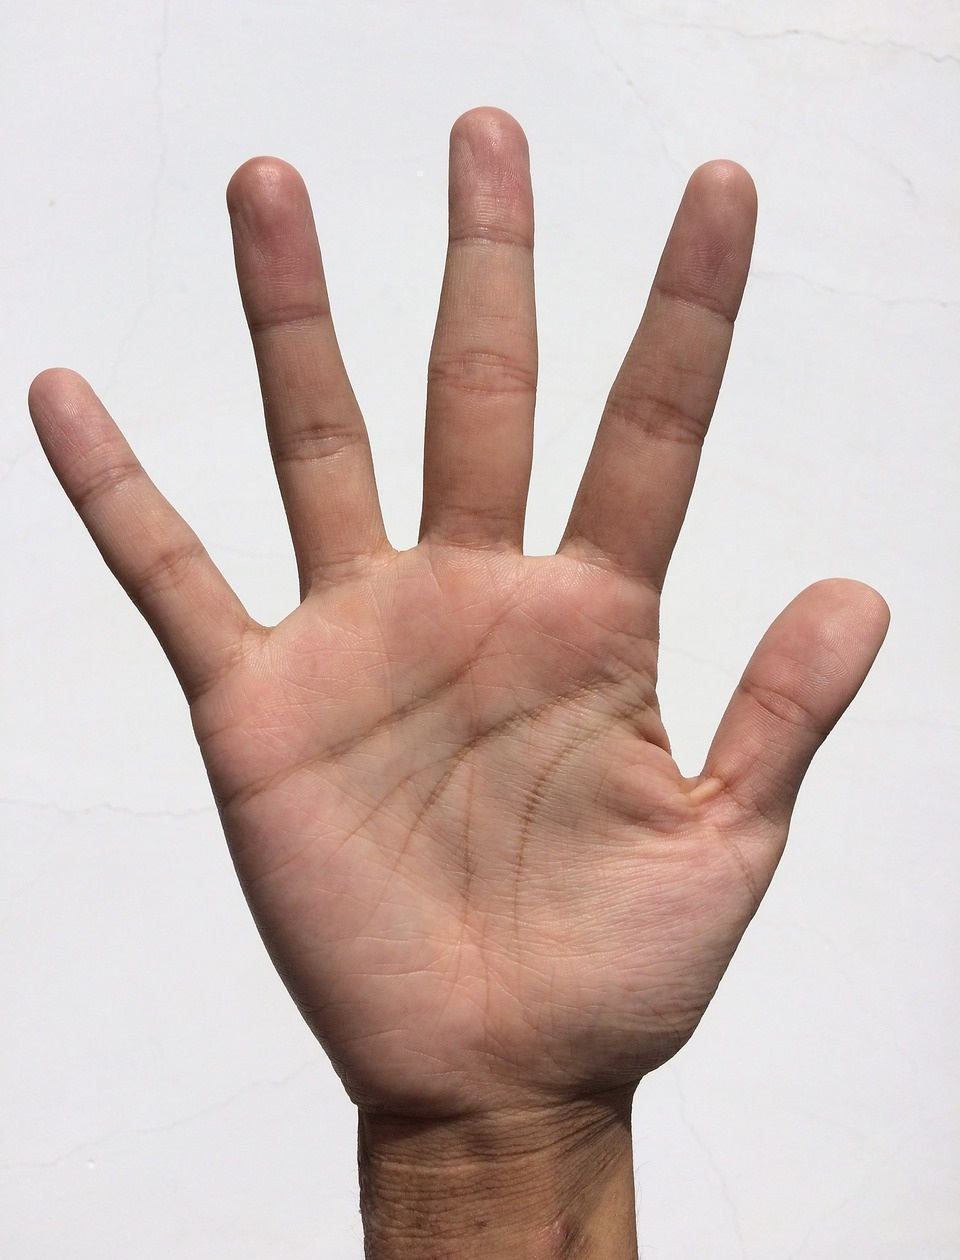
\includegraphics[scale=.20]{3/.report/blending/et/hand.png}
      \caption{Merge}
    \endminipage \hfill
    \end{figure}
    
    \begin{figure}[!htb]
    \minipage{0.5\textwidth}
      \fbox{
\includegraphics[scale=.20]{3/.report/blending/et/mask.png}}
      \caption{Merger}
    \endminipage \hfill
    %
    \minipage{0.5\textwidth}
      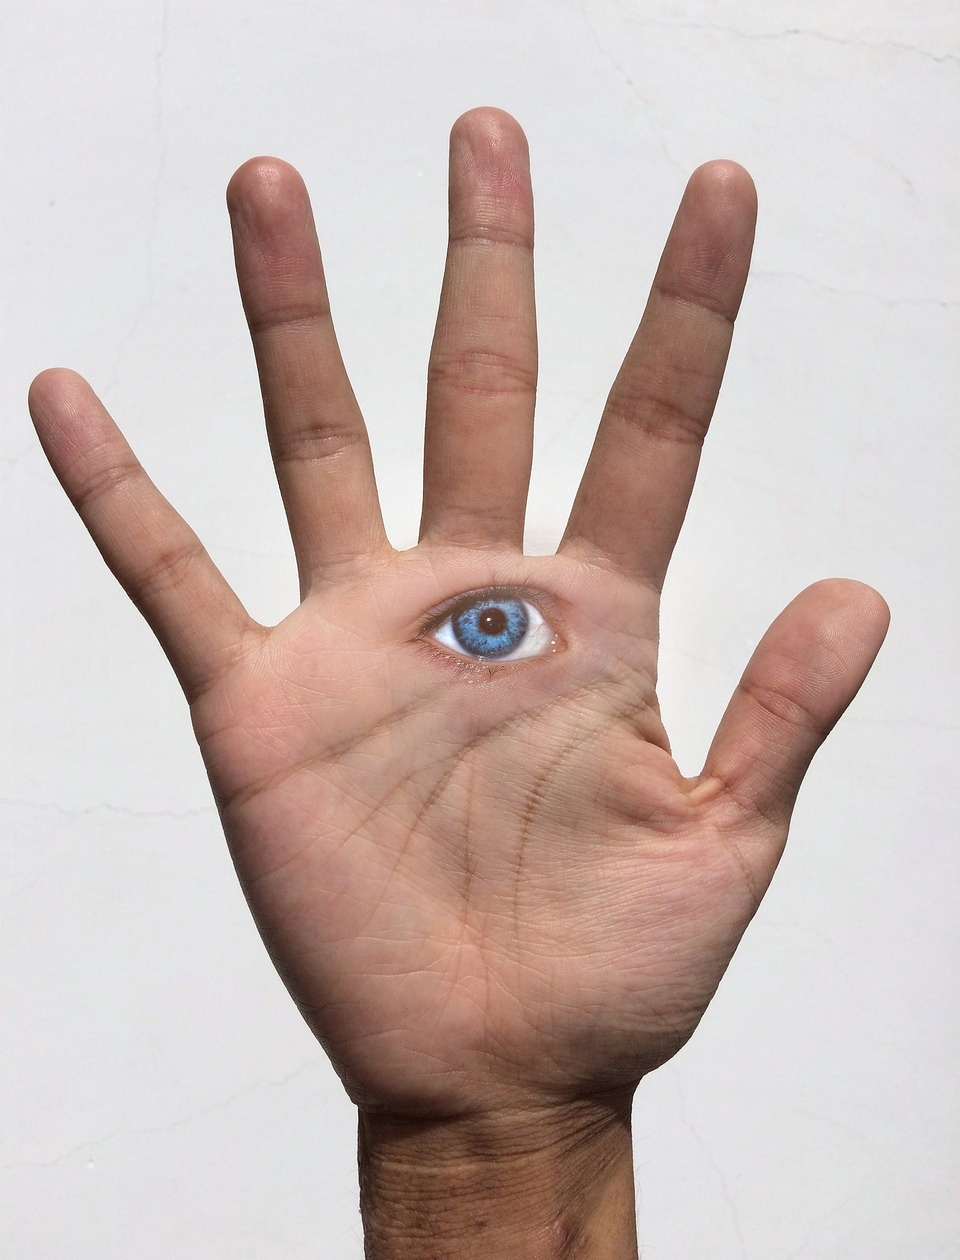
\includegraphics[scale=.20]{3/.report/blending/et/blend.png}
      \caption{Merge}
    \endminipage \hfill
    %
    \end{figure}
% ------------------------------------------------------- 
    \pagebreak
% -------------------------------------------------------
% Denoising
    \subsection*{Denoising}
    Since noise only adds to the detail of the image (not the approximation), we can very well reduce the noise in the image by working with the detail-levels in transforms and pyramids. Using this idea (usually with coefficient cutoff-thresholding), I tried to denoise some images. Results are presented below.\\[1pt]
    
    \textbf{Image}: Barbara  \textbf{Type}: Continuous (Real World Image)\\

    \begin{figure}[!htb]
    \minipage{0.45\textwidth}
      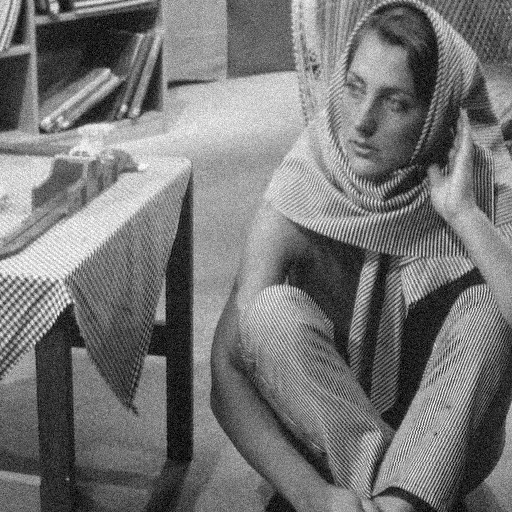
\includegraphics[scale=0.4]{./denoising/b/b05.png}
      \caption{Noisy Image}
    \endminipage \hfill
    \minipage{0.45\textwidth}
      \includegraphics[scale=.4]{./denoising/b/p_1_0_013.png}
      \caption{Pyramid Denoising}
    \endminipage
    \end{figure}\\
    

    \begin{figure}[!htb]
    \minipage{0.45\textwidth}
      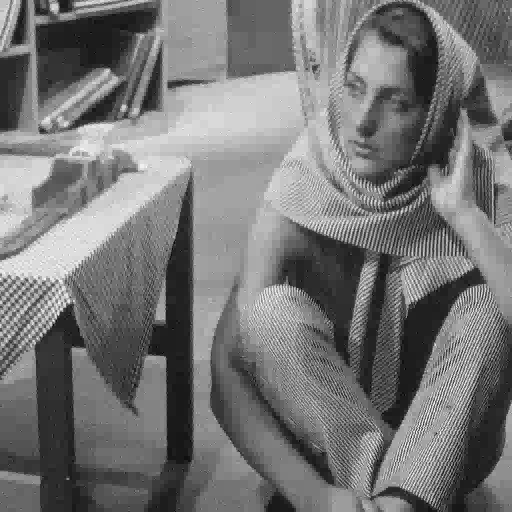
\includegraphics[scale=0.4]{./denoising/b/hard0_15.png}
      \caption{Hard Denoising}
    \endminipage \hfill
    \minipage{0.45\textwidth}
      \includegraphics[scale=.4]{./denoising/b/smooth0_05.png}
      \caption{Soft Denoising}
    \endminipage
    \end{figure}
    \pagebreak

%---------------------------------------------
    
    \pagebreak
    \textbf{Image}: Shepplogan  \textbf{Type}: Discrete (Cartoon Image)\\
    
    \begin{figure}[!htb]
    \minipage{0.45\textwidth}
      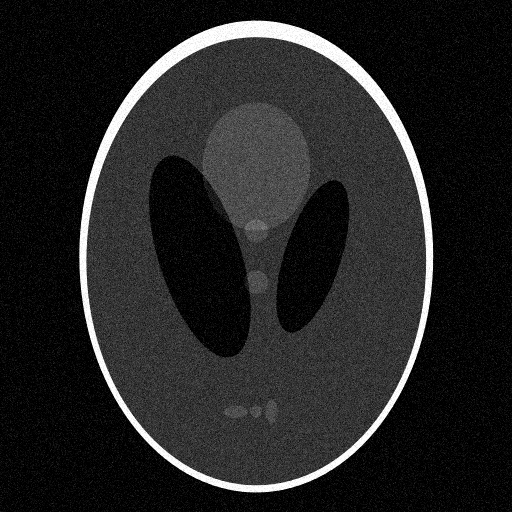
\includegraphics[scale=0.4]{./denoising/n/n05.png}
      \caption{Noisy Image}
    \endminipage \hfill
    \minipage{0.45\textwidth}
      \includegraphics[scale=.4]{./denoising/n/p_1_0_013.png}
      \caption{Pyramid Denoising}
    \endminipage
    \end{figure}
    

    \begin{figure}[!htb]
    \minipage{0.45\textwidth}
      
\includegraphics[scale=0.4]{./denoising/n/hard0_05.png}
      \caption{Hard Denoising}
    \endminipage \hfill
    \minipage{0.45\textwidth}
      \includegraphics[scale=.4]{./denoising/n/smooth0_05.png}
      \caption{Soft Denoising}
    \endminipage
    \end{figure}
    
    \textbf{Observation}\\
    It was observed that the transform based denoising worked much better than thresholding using laplacian pyramids. Also, denoising worked much better in the case of discrete image, than continuous one. Also, though slight, there was a subtle difference between soft and hard denoising, with soft being more smooth (or acceptable).
    
    
    \pagebreak

%--------------------------------------------- 
% Compression
    \subsection*{Compression}
    We can achieve (lossy) image compression by letting go of smaller detail-coefficients, with thresholding. This allows us to reduce the size, with some sacrifice to the image quality.
    \\Also, we could now encode the image using run-length encoding as detail coefficients are very close to zero, and with cut-off, mostly zero. I tried compression with some images. Results are presented below.\\[2pt]
    \textbf{Image}: Barbara  \textbf{Type}: Continuous (Real World Image)\\
    \begin{figure}[!htb]
    \minipage{0.45\textwidth}
      \includegraphics[scale=0.4]{./compression/1/20.png}
      \caption{K = 20, Size = 154KB}
    \endminipage \hfill
    \minipage{0.45\textwidth}
      \includegraphics[scale=.4]{./compression/1/50.png}
      \caption{K = 50, Size = 29KB}
    \endminipage
    \end{figure}
    

    \begin{figure}[!htb]
    \minipage{0.45\textwidth}
      \includegraphics[scale=0.4]{./compression/1/80.png}
      \caption{K = 80, Size = 15KB}
    \endminipage \hfill
    \minipage{0.45\textwidth}
      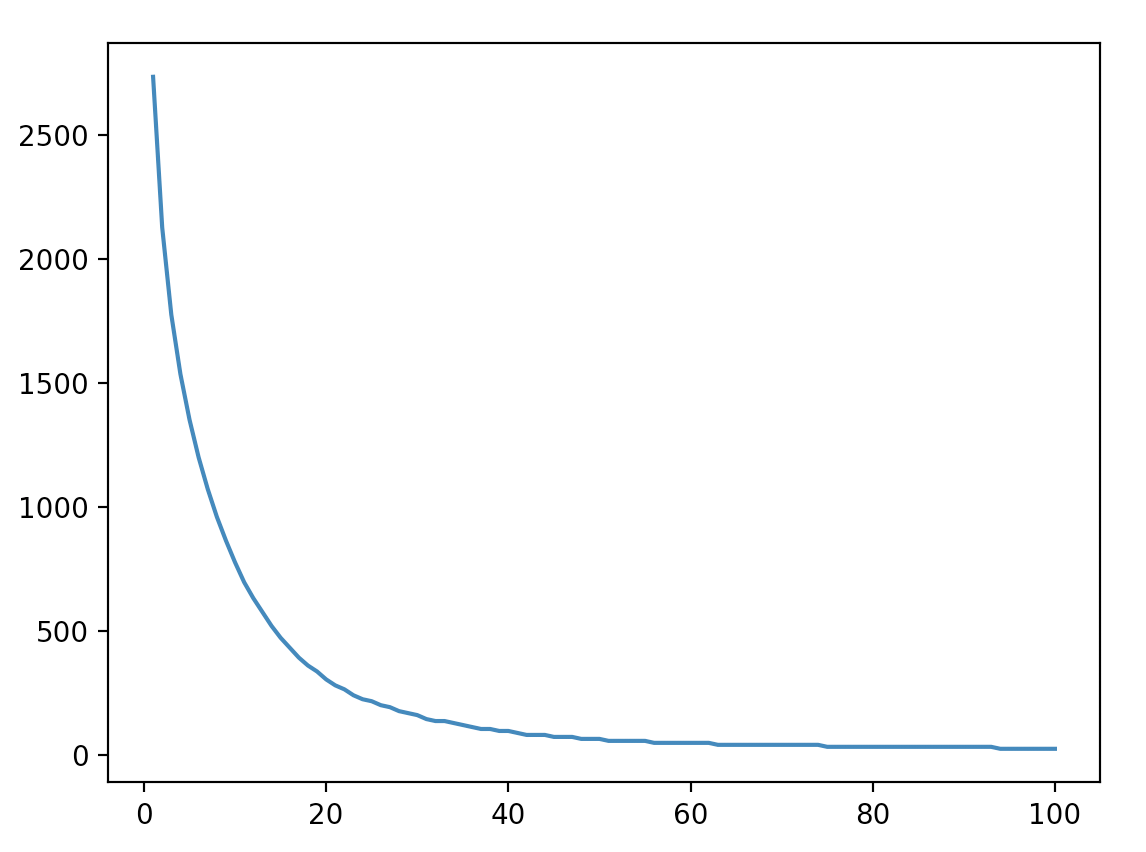
\includegraphics[scale=.4]{./compression/plots/b.png}
      \caption{Plot of binary-size vs. K}
    \endminipage
    \end{figure}
    
%------------------------------------
    \pagebreak
    \textbf{Image}: Shepplogan  \textbf{Type}: Discrete (Cartoon Image)\\
    \begin{figure}[!htb]
    \minipage{0.45\textwidth}
      \includegraphics[scale=0.4]{./compression/2/20.png}
      \caption{K = 20, Size = 67KB}
    \endminipage \hfill
    \minipage{0.45\textwidth}
      \includegraphics[scale=.4]{./compression/2/50.png}
      \caption{K = 50, Size = 32KB}
    \endminipage
    \end{figure}
    

    \begin{figure}[!htb]
    \minipage{0.45\textwidth}
      \includegraphics[scale=0.4]{./compression/2/80.png}
      \caption{K = 80, Size = 18KB}
    \endminipage \hfill
    \minipage{0.45\textwidth}
      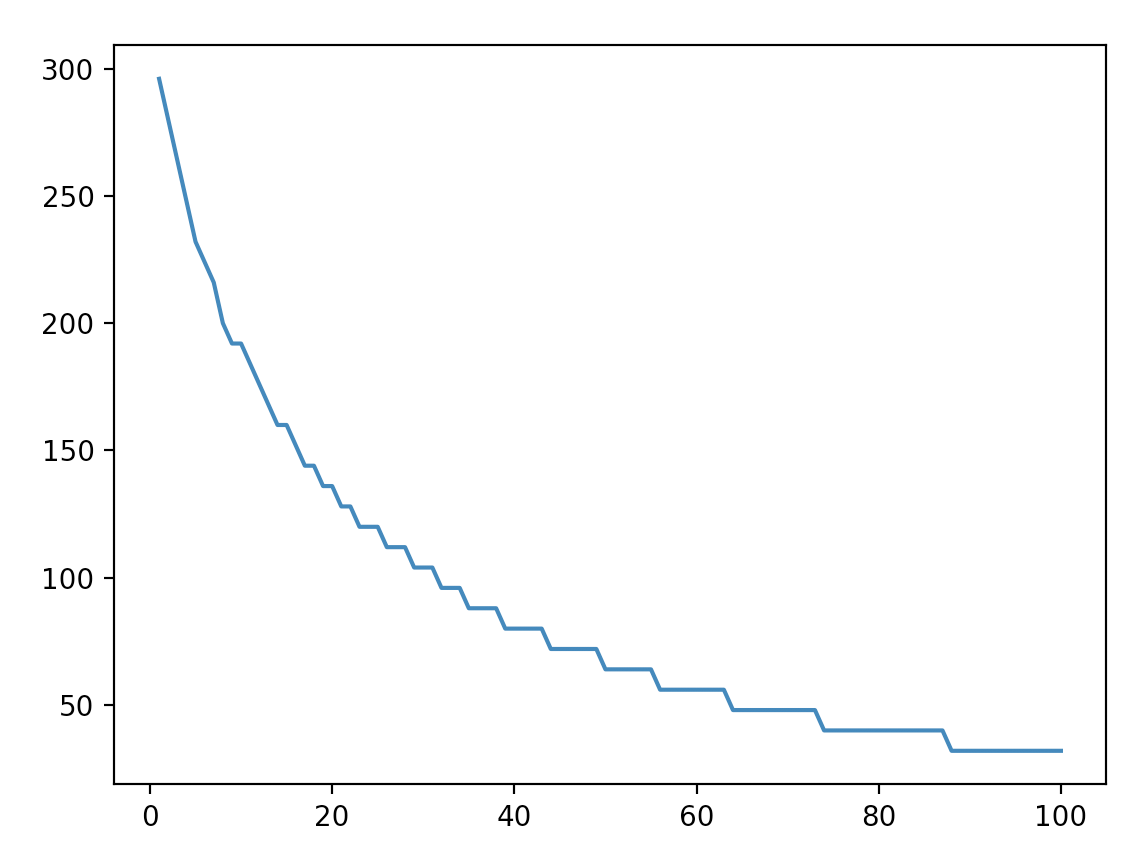
\includegraphics[scale=.4]{./compression/plots/c.png}
      \caption{Plot of binary-size vs. K}
    \endminipage
    \end{figure}

    \textbf{Observation}\\
    I feel, nice compression ratios were achieved :)\\
    Also, it was observed, that in the case of a continuous real world image, the compression increased phenomenally initially, and then slowed down as mostly coarse values remained. In the case of discrete image, instead, the starting value was already very small and the progression in compression was relatively slow, this maybe because most of the detail-coefficients are already small.
    
%--------------------------------------------- 
\pagebreak
%---------------------------------------------
% Bonus
\subsection*{Wavelets with Lifting Scheme}
I implemented the wavelet-transform, as deescribed in the paper provided.\\
This wavelet transform, is based on piece-wise linear approximation and wavelet functions. Unlike Haar-Transform, the transform focuses on linearity-correlation b/w contigious coefficients. This allows it to preserve linear variation very efficiently.\\
Also, since the transform is bi-orthogonal, all the coefficients (approximating and detailing) were given the same weightage. This made denoising and compression very difficult. To counter that, I also implemented another form, where there is scaling b/w levels leading to better results, these are presented here.\\
Another note (also an observation) is that Haar-Transform performs better than this transform on discrete (cartoon-type) images, because its key-functions are all constant functions. In the case of continuous images, the new transform performed much better.\\
\subsubsection*{Denoising}

    \begin{figure}[!htb]
    \minipage{0.45\textwidth}
      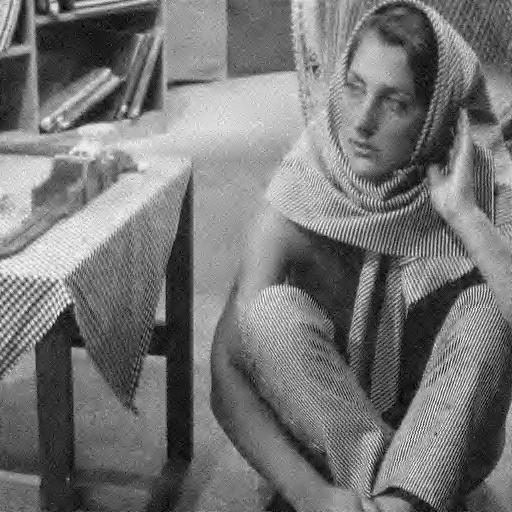
\includegraphics[scale=0.4]{3/.report/denoising/bn/0_0_125000.jpg}
      \caption{Continuous}
    \endminipage \hfill
    \minipage{0.45\textwidth}
      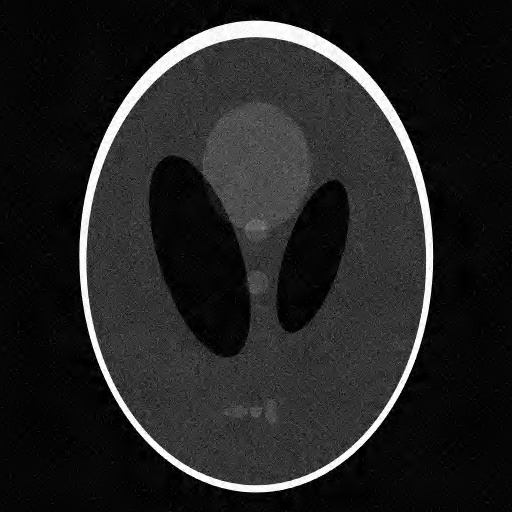
\includegraphics[scale=.4]{3/.report/denoising/bn/0_0_097500.jpg}
      \caption{Discrete}
    \endminipage
    \end{figure}

\pagebreak
\subsubsection*{Compression}

    \textbf{Image}: Boat  \textbf{Type}: Continuous\\
    \begin{figure}[!htb]
    \minipage{0.45\textwidth}
      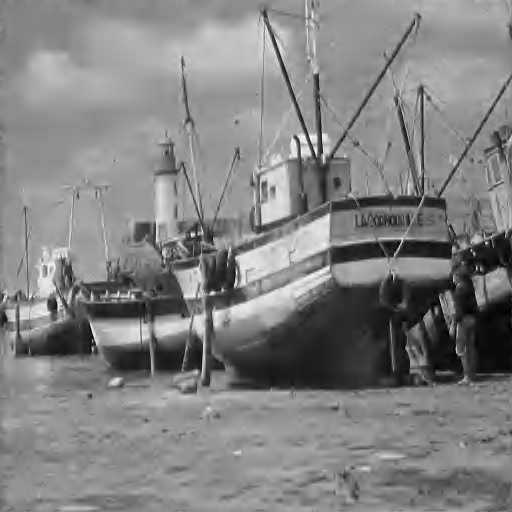
\includegraphics[scale=0.4]{3/.report/compression/3/15.png}
      \caption{K = 15}
    \endminipage \hfill
    \minipage{0.45\textwidth}
      \includegraphics[scale=.4]{./compression/3/50.png}
      \caption{K = 50}
    \endminipage
    \end{figure}
    
    \begin{figure}[!htb]
    \minipage{0.45\textwidth}
      \includegraphics[scale=0.4]{./compression/3/80.png}
      \caption{K = 80}
    \endminipage \hfill
    \minipage{0.45\textwidth}
      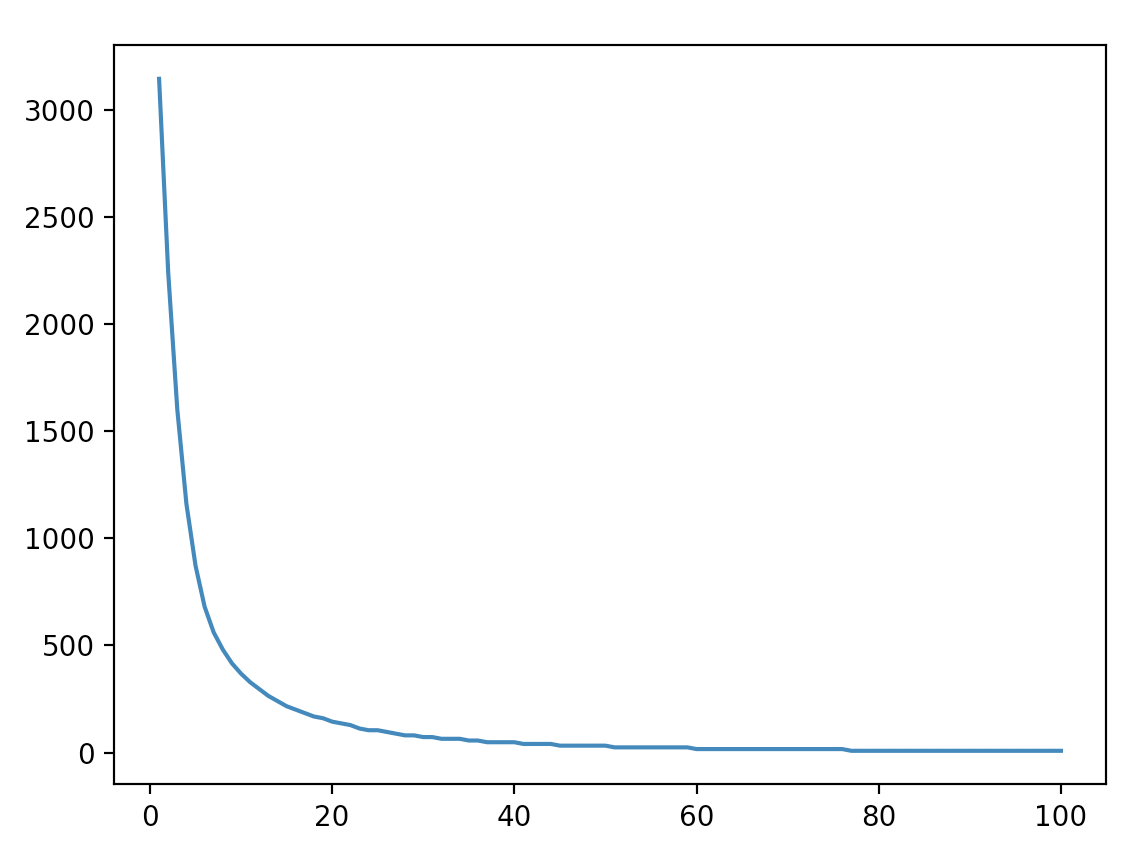
\includegraphics[scale=.4]{./compression/plots/bn.png}
      \caption{Plot of binary-size vs. K}
    \endminipage
    \end{figure}
    \\
    \textbf{Comment}\\
    Lifting-lazy scheme transform lost image clarity very early on, but still around smaller values of K, both image clarity and size were very well related (as good as jpeg).

%--------------------------------------------- 
\pagebreak
%---------------------------------------------
% Summary
\subsection*{Summary}
    This assignment was very interesting, and I learnt a lot of new things. What was discussed in class was very helpful. \\
    Thanks and Regards\\
    Rajbir
\end{document}